\documentclass[12pt,a4paper]{article}

\usepackage{amsmath,amssymb,amsfonts}
\usepackage{geometry}
\usepackage[colorlinks=true,linkcolor=red!70!black,citecolor=green!50!black,urlcolor=blue!80!black]{hyperref}
\usepackage{booktabs}
\usepackage{physics}
\usepackage{xcolor}
\usepackage{graphicx}
\usepackage{tabularx}
\usepackage{natbib}
\usepackage{enumitem}
\newcommand{\prd}{Phys.\ Rev.\ D}

\geometry{margin=2.5cm}


% ─── Macros SSEE ────────────────────────────────────────────────────────────
\newcommand{\phiG}{\varphi}
\newcommand{\KAL}{\mathrm{KAL}_0}
\newcommand{\MIRA}{\mathcal{M}}
\newcommand{\AURA}{\mathcal{A}}
\newcommand{\Mpl}{M_{\mathrm{Pl}}}
\newcommand{\Omde}{\Omega_{\mathrm{DE}}}  % fraccion de densidad (solo en z_*)
\newcommand{\Omm}{\Omega_{m}}
\newcommand{\half}{\tfrac{1}{2}}
\newcommand{\Hzero}{H_0}
\newcommand{\bc}{\beta_c}
\newcommand{\fsc}{f_{\mathrm{screen}}}
\newcommand{\sK}{s_K}          % dilucion de PRESION; NO es alpha_K
\newcommand{\sDE}{s_{\mathrm{DE}}} % saturacion = |w_0|; NO es 1-Omega_m
\newcommand{\alphaK}{\alpha_K}     % kineticidad Bellini-Sawicki (P7)
\renewcommand{\Omega}{\varOmega}
% ─────────────────────────────────────────────────────────────────────────────

\title{\textbf{SSEE and the Hubble Tension:\\
       An Algebraic Local Screening Fraction}}

\author{Mike Edison Almeida Vallejo\\
        \small\texttt{mike.almeida1721@gmail.com}}

\date{May 2026 --- Paper 9 of the SSEE series}

\sloppy
% ACTA-PROCEDENCIA {"commit": "5651fc97a90dc17d52be0317b46142db9ac86fcb", "reproducible_desde_commit": true, "cambios_sin_commitear": [], "script": "src/valores_tex.py", "script_sha256": "cb5ceb2369bdef5e586d471d57d44a11a9fed354be540a96ce34da85e582efa4", "nucleo_sha256": "5cec8af72d88f154116c5a532e42a9b6ff7a5b4c3d86bcc6921eabb246698993", "entradas": {"manuscript/valores.yaml": "5fa01e91dd68164243d664a73264bb6c87431d2ec0bd69db87c62a983a55992d", "results/logs/kids_publicados.json": "6c25c98059ce91038215358b4e7ac9cfb40198f410354937cee4ea00b46654ff", "results/logs/p10_uv_fscreen.json": "8fb68b295c848e0292e5701e7de795ba7c7ba25e3292d776260bb3dea8970c95", "results/logs/s8_desde_b1.json": "6d225f4403fbfbe6934d7edca26aaefbbe19e05ef6c7b7eda842a259e798b1c1"}, "argv": ["src/valores_tex.py"], "fecha": "2026-09-30T19:35:24", "host": "mike-System-Product-Name", "python": "3.12.3", "versiones": {}, "nucleos": {"OMP_NUM_THREADS": null, "MKL_NUM_THREADS": null, "OPENBLAS_NUM_THREADS": null, "OMPI_COMM_WORLD_SIZE": null}}
% GENERADO por src/valores_tex.py desde manuscript/valores.yaml — NO EDITAR A MANO.
% Cada numero sale de un log de la cadena de procedencia (dvc.yaml + acta).
\providecommand{\val}[1]{\csname ssee@val@#1\endcsname}
\expandafter\def\csname ssee@val@H0_glob\endcsname{67.962142}  % results/logs/p10_uv_fscreen.json#H0_glob
\expandafter\def\csname ssee@val@PTE_k1000_lcdm\endcsname{0.010}  % results/logs/kids_publicados.json#PTE.lcdm.PTE
\expandafter\def\csname ssee@val@PTE_k1000_ssee\endcsname{0.012}  % results/logs/kids_publicados.json#PTE.ssee.PTE
\expandafter\def\csname ssee@val@S8_b1_lcdm\endcsname{0.8229}  % results/logs/s8_desde_b1.json#filas.LCDM.S8
\expandafter\def\csname ssee@val@S8_b1_lcdm_sigma\endcsname{0.0059}  % results/logs/s8_desde_b1.json#filas.LCDM.S8_sigma
\expandafter\def\csname ssee@val@S8_b1_ssee\endcsname{0.8261}  % results/logs/s8_desde_b1.json#filas.SSEE.S8
\expandafter\def\csname ssee@val@S8_b1_ssee_sigma\endcsname{0.0054}  % results/logs/s8_desde_b1.json#filas.SSEE.S8_sigma
\expandafter\def\csname ssee@val@S8_legacy_dato\endcsname{0.8265}  % results/logs/kids_publicados.json#kids_legacy.S8
\expandafter\def\csname ssee@val@S8_legacy_dato_sigma\endcsname{0.0176}  % results/logs/kids_publicados.json#kids_legacy.S8_sigma
\expandafter\def\csname ssee@val@chi2_k1000_lcdm\endcsname{262.75}  % results/logs/kids_publicados.json#PTE.lcdm.chi2
\expandafter\def\csname ssee@val@chi2_k1000_publicado\endcsname{260.31}  % results/logs/kids_publicados.json#kids1000_maxpost.chi2
\expandafter\def\csname ssee@val@chi2_k1000_ssee\endcsname{265.44}  % results/logs/kids_publicados.json#PTE.ssee.chi2
\expandafter\def\csname ssee@val@dAIC_k1000\endcsname{-5.31}  % results/logs/kids_publicados.json#seleccion_kids1000.delta_AIC
\expandafter\def\csname ssee@val@dBIC_k1000\endcsname{-19.0}  % results/logs/kids_publicados.json#seleccion_kids1000.delta_BIC
\expandafter\def\csname ssee@val@dchi2_k1000\endcsname{2.69}  % results/logs/kids_publicados.json#seleccion_kids1000.delta_chi2
\expandafter\def\csname ssee@val@fscreen_IR\endcsname{0.067253}  % results/logs/p10_uv_fscreen.json#f_screen_IR
\expandafter\def\csname ssee@val@fscreen_UV_corr\endcsname{0.002268}  % results/logs/p10_uv_fscreen.json#f_screen_UV_corr
\expandafter\def\csname ssee@val@fscreen_full\endcsname{0.069522}  % results/logs/p10_uv_fscreen.json#f_screen_full
\expandafter\def\csname ssee@val@logA_b1_lcdm\endcsname{3.045}  % results/logs/s8_desde_b1.json#filas.LCDM.logA
\expandafter\def\csname ssee@val@logA_b1_ssee\endcsname{3.042}  % results/logs/s8_desde_b1.json#filas.SSEE.logA
\expandafter\def\csname ssee@val@logA_b1_ssee_sigma\endcsname{0.013}  % results/logs/s8_desde_b1.json#filas.SSEE.logA_sigma
\expandafter\def\csname ssee@val@p_dchi2_k1000\endcsname{0.61}  % results/logs/kids_publicados.json#seleccion_kids1000.p_delta_chi2
\expandafter\def\csname ssee@val@sK_IR\endcsname{0.403302}  % results/logs/p10_uv_fscreen.json#s_K_IR
\expandafter\def\csname ssee@val@sK_UV_corr\endcsname{0.013603}  % results/logs/p10_uv_fscreen.json#s_K_UV_corr
\expandafter\def\csname ssee@val@sK_full\endcsname{0.416905}  % results/logs/p10_uv_fscreen.json#s_K_full
\expandafter\def\csname ssee@val@tension_b1_lcdm\endcsname{2.59}  % results/logs/s8_desde_b1.json#filas.LCDM.tension_kids
\expandafter\def\csname ssee@val@tension_b1_ssee\endcsname{2.73}  % results/logs/s8_desde_b1.json#filas.SSEE.tension_kids
\expandafter\def\csname ssee@val@z_k1000_lcdm\endcsname{2.5}  % results/logs/kids_publicados.json#PTE.lcdm.z
\expandafter\def\csname ssee@val@z_k1000_ssee\endcsname{2.4}  % results/logs/kids_publicados.json#PTE.ssee.z

\begin{document}
\maketitle

\begin{abstract}
The Hubble tension between the CMB-inferred value $H_0^{\rm CMB} = 67.4\pm0.5$
km/s/Mpc and the local distance-ladder measurement $H_0^{\rm SH0ES} = 73.04\pm1.04$
km/s/Mpc remains one of the sharpest anomalies in modern cosmology.
Within the Structural Self-Energy Expansion (SSEE) framework, the algebraic
constants $\phiG$ (golden ratio) and $\pi$ determine all parameters with zero
free parameters.
We derive algebraically that the dark-energy EFT of Paper~7 and the disformal
geodesic of Paper~8 together imply a \emph{local screening fraction}
\[
  \fsc \;=\; \frac{\sK}{3\,\MIRA}
       \;=\; \frac{\pi - \phiG}{(\phiG+\pi)^2}
       \;\approx\; 0.06725\,,
\]
where $\sK = 3\,\sDE(1+w_0) = -3w_0(1+w_0)$ is the pressure-dilution rate
derived from the
background equation of state, and $\MIRA = \bc/2 = (3\phiG+\pi)/4 \approx \val{MIRA_d4}$
is the effective optical coupling derived from the disformal null geodesic.
The two structural constants $\AURA = 2\MIRA$ cancel exactly in the ratio,
leaving a pure function of $\phiG$ and $\pi$.
The lens is applied in the direction set by what is measured. The only
directly measured expansion rate is the local one,
$H_0^{\rm SH0ES} = 73.04\pm1.04$\,km\,s$^{-1}$\,Mpc$^{-1}$
(Riess et al.\ 2022); it enters, and the global background rate comes out,
\[
  H_0^{\rm glob,IR} \;=\; H_0^{\rm SH0ES}\,(1-\fsc^{\rm IR})
                 \;=\; 73.04\times(1-0.06725)
                 \;=\; 68.13 \text{ km/s/Mpc}\,,
\]
to be compared with the dimensionless algebraic number
$3(\phiG+\pi)^2 = 67.96214$ (Postulate~D, Paper~1): a residual of $0.166$,
i.e.\ $0.17\sigma$, with \emph{zero free parameters}.
\footnote{\label{fn:regime}\textbf{Regime, stated once for the whole paper.} This paper works
in the \emph{infrared} regime ($M\to\infty$), where $\sK=\sK^{\rm IR}=\val{S_K_d6}$
and hence $\fsc=0.06725$.  The screening fraction of the full theory is not a
separate quantity but the \emph{sum} of this term and the ultraviolet
correction supplied by Paper~10, $\sK^{\rm full}=\sK^{\rm IR}+\val{sK_UV_corr}=\val{sK_full}$,
giving $\fsc^{\rm full}=\fsc+\val{fscreen_UV_corr}=\val{fscreen_full}$ and the single model value
$H_0^{\rm glob}=73.04\times(1-\val{fscreen_full})=\val{H0_glob}$~km/s/Mpc.  There is
therefore \emph{one} $H_0^{\rm glob}$, not an infrared one and an ultraviolet
one: the $68.13$ used throughout this paper is the same cascade evaluated with
the infrared term alone, and it is superseded by the complete value once the
ultraviolet completion is included.  In either case the propagated uncertainty
($\pm0.970$ in the infrared regime, $\pm0.968$ with the full screening fraction), inherited from the SH0ES input, dominates over the residual
against the pure number.}
The comparison is a
coincidence of value, not an identity: $3(\phiG+\pi)^2$ is a pure number and
carries no units, whereas $H_0^{\rm glob}$ inherits km\,s$^{-1}$\,Mpc$^{-1}$
from the measurement. The agreement is therefore an output of the cascade,
never its input.
This adopts the single algebraic target $3(\phiG+\pi)^2$ shared by every sector
of the suite (2026 reframe). The earlier register used the CMB-mapped value
$H_0^{\rm MIRA}=67.037$, giving $H_0^{\rm local}=71.87$ ($1.12\sigma$); this is now
superseded. The 2026 $\omega_m$-direct reframe adopts the single algebraic anchor
$3(\varphi+\pi)^2=\val{H0_ALG_d5}$ as the algebraic target shared by all
sectors --- with \emph{no} matter factor, the CMB density following as
$\Omega_{m,\rm CMB}=\omega_m/h^2$ (Paper~1).
The correction operates at late times ($z < 0.15$) through the scalar kinetic
energy contribution to the local expansion rate, and does not modify the
sound horizon $r_d$, the CMB peak positions, or the growth factor $\sigma_8$
derived in Papers~3 and~5.
The UV completion of Paper~10 sharpens the residual to
$4.2\times10^{-6}$ ($H_0^{\rm glob,UV} = \val{H0_GLOBAL_d5}$), the small-scale
refinement of the same cascade.
\end{abstract}

\clearpage
{\small\tableofcontents}
\clearpage

%% ─────────────────────────────────────────────────────────────────────────────
\section{Introduction}
\label{sec:intro}
%% ─────────────────────────────────────────────────────────────────────────────

The Hubble tension \citep{Verde2019,Riess2022,Kamionkowski2023,DiValentino2021,Knox2020}
is the $4$--$6\sigma$ discrepancy between measurements of the present expansion
rate obtained by two independent methods:
\begin{itemize}
  \item \textbf{Early-universe inference}: CMB anisotropies (Planck~PR4,
        \citealt{Planck2020}) combined with acoustic oscillation physics
        yield $H_0 = 67.4\pm0.5$ km/s/Mpc under the assumption of
        $\Lambda$CDM.
  \item \textbf{Local distance-ladder}: Type~Ia supernovae
        \citep{Riess1998,Perlmutter1999} calibrated with
        Cepheids in the SH0ES programme \citep{Riess2019,Riess2022} give
        $H_0 = 73.04\pm1.04$ km/s/Mpc, probing predominantly $z < 0.15$.
\end{itemize}

The SSEE framework \citep{Paper1,Paper2,Paper3,Paper7} derives the
cosmological expansion rate algebraically:
\begin{equation}
  \Hzero^{\rm alg} \;=\; 3(\phiG+\pi)^2 \;\approx\; \val{H0_ALG_d5}\;\text{km/s/Mpc}\,,
  \label{eq:H0alg}
\end{equation}
which agrees with Planck at the $1.1\sigma$ level
\citep{Paper2} but does not, at first sight, resolve the local tension.

In this paper we show that the same algebraic structure that produces
$\Hzero^{\rm alg}$ also produces a local kinematic correction
$\fsc \approx 0.06725$ from the SSEE algebra. Applied to the measured
local rate $H_0^{\rm SH0ES} = 73.04\pm1.04$~km/s/Mpc, this returns a global
background rate $H_0^{\rm glob,IR} = 68.13$ km/s/Mpc in the IR regime, to be
compared with the algebraic number $3(\phiG+\pi)^2 = 67.96214$ ($0.17\sigma$);
the model value, with the complete $\fsc$, is $67.96214$ km/s/Mpc (footnote~\ref{fn:regime}).
The derivation combines two results already established in this series:
\begin{enumerate}
  \item From Paper~7 \citep{Paper7}: the pressure-dilution rate
        $\sK = 3\,\sDE(1+w_0)$, which follows from the background
        Friedmann equations and the $k$-essence action $K(X) = X/\KAL$.
  \item From Paper~8 \citep{Paper8}: the effective optical coupling
        $\MIRA = \bc/2 = (3\phiG+\pi)/4$, which emerges from the disformal
        null geodesic of dark matter.
\end{enumerate}
Together these give the exact algebraic identity $\fsc = \sK/(3\MIRA)$.

\bigskip

\noindent\textbf{Organisation.}
Section~\ref{sec:background} recalls the key results from Papers~7 and~8.
Section~\ref{sec:identity} derives the algebraic identity in three steps.
Section~\ref{sec:mechanism} interprets the result physically.
Section~\ref{sec:consistency} verifies consistency with the rest of the
SSEE series.
Section~\ref{sec:prediction} states the pre-committed falsifiable prediction
and its current observational status.
Section~\ref{sec:comparison} compares the mechanism quantitatively against
early dark energy, self-interacting dark radiation, and late dark-energy
transitions.
Section~\ref{sec:conclusions} summarises.

%% ─────────────────────────────────────────────────────────────────────────────
\section{Background: EFT Kineticity and Disformal Coupling}
\label{sec:background}
%% ─────────────────────────────────────────────────────────────────────────────

\subsection{The SSEE action (Paper 7)}
\label{sec:p7recap}

The fundamental action of SSEE is a $k$-essence scalar
\citep{ArmendarizPicon1999,ArmendarizPicon2001} minimally
coupled to gravity and conformally coupled to dark matter:
\begin{equation}
  S = \int d^4x\,\sqrt{-g}\,\left[
      \frac{\Mpl^2}{2}R + K(X,\phi) + \mathcal{L}_m
      \right]\,,
  \label{eq:action}
\end{equation}
with kinetic kernel
\begin{equation}
  K(X,\phi) = \frac{X}{\KAL} + \frac{X^2}{M^4} - V_0\,e^{-\lambda\phi/\Mpl}\,,
  \label{eq:Kkernel}
\end{equation}
where $X = -\tfrac{1}{2}g^{\mu\nu}\partial_\mu\phi\,\partial_\nu\phi$ and
\begin{align}
  \KAL   &= \frac{\phiG+\pi}{2}+\pi \approx 5.521\,, \label{eq:KAL}\\
  \bc \equiv \AURA &= \frac{3\phiG+\pi}{2} \approx 3.998\,. \label{eq:bc}
\end{align}
All parameters are algebraically fixed; no fitting is performed.

The dark-energy equation-of-state parameters derived in Paper~1 are
\begin{align}
  w_0 &= -\frac{\AURA}{\phiG+\pi} \approx -0.840\,, \label{eq:w0}\\
  \sDE &= -w_0 = \frac{\AURA}{\phiG+\pi} = \val{S_DE_d6}\,. \label{eq:sDE}
\end{align}

The quantity entering the screening fraction is the fractional dilution rate
of the dark-energy \emph{pressure} per e-fold,
\begin{equation}
  \sK \;\equiv\; -\frac{1}{\rho_\phi}\frac{dp_\phi}{dN}
      \;=\; -3w_0(1+w_0)\,, \qquad N = \ln a,
  \label{eq:sK_def}
\end{equation}
which carries only the equation of state: no factor of $H$, no density, and
no kinetic function.  Section~\ref{sec:identity} gives its exact algebraic
form.

\paragraph{A label corrected.}
Earlier versions of this paper called this quantity $\alphaK$ and defined it
as the Bellini--Sawicki kineticity $2XK_X/(\Mpl^2H^2)$
\citep{Bellini2015,Gubitosi2013,Gleyzes2013}.  That identification was wrong,
and it matters here rather than being a matter of notation.  The kineticity of
the SSEE action is $\alphaK = 3(1-\Omega_m)(5-3w_0) = \val{alpha_K_z0_d6}$ (Paper~7,
verified against \textsc{hi\_class}); it depends on $K(X)$ and it evolves.
The constant $\val{S_K_d6}$ is $\sK$, and the distinction is what makes
$\fsc$ well defined: a screening fraction built from a kineticity would
inherit that kineticity's dependence on the expansion history, while one built
from $\sK$ cannot, because $\sK$ contains no $H$ (§\ref{sec:step4}).

\subsection{The disformal coupling and MIRA (Paper 8)}
\label{sec:p8recap}

Paper~8 extends the action to the strong-gravity regime by coupling dark
matter to the disformal metric \citep{Bekenstein1993,Zumalacarregui2014}
\begin{equation}
  \tilde{g}_{\mu\nu} = g_{\mu\nu} + \frac{2}{M^4}\,\partial_\mu\phi\,\partial_\nu\phi\,.
  \label{eq:disformal}
\end{equation}
The disformal null geodesic for a photon passing through a dark-matter halo
yields a total deflection angle
\begin{equation}
  \hat\alpha_{\rm total} \approx \bc\,\left(\frac{4GM}{c^2 b}\right)\,,
  \label{eq:deflection}
\end{equation}
where $b$ is the impact parameter and $\bc = \AURA$.
The effective Einstein ring radius is therefore amplified by
\begin{equation}
  \frac{\theta_E^{\rm SSEE}}{\theta_E^{\rm GR}} \approx \sqrt{\bc} \approx \MIRA\,,
  \qquad
  \MIRA \equiv \frac{\bc}{2} = \frac{3\phiG+\pi}{4} \approx \val{MIRA_d4}\,.
  \label{eq:MIRA_def}
\end{equation}
The constant $\MIRA$ encodes the effective optical coupling of the disformal
sector; it is not a fitted parameter but derived from $\bc = \AURA$.
Following the 2026 $\omega_m$-direct reframe (OP-8 dissolved), $\MIRA$ is
\emph{not} identified with the CMB-to-dynamical matter ratio (which is
it is not identified with any matter ratio: there is one matter density,
$\Omega_m=\val{OMEGA_M_TOTAL_d6}$, and $s_m=\val{S_M_d6}$ is a number of the equation of state,
so the $\approx1.93$ that earlier drafts formed between them divided objects of
different kinds);
it is fixed algebraically by $\bc=\AURA$ and realised physically as the
Hubble screening amplitude derived below.

%% ─────────────────────────────────────────────────────────────────────────────
\section{Algebraic Derivation: $\fsc = \sK/(3\MIRA)$}
\label{sec:identity}
%% ─────────────────────────────────────────────────────────────────────────────

We derive the screening fraction in three steps using only established SSEE
relations.  Scalar screening mechanisms of this type were introduced by
\citet{Vainshtein1972} and reviewed in \citet{Babichev2013}; the SSEE
realisation is a kinematic analogue arising from the k-essence EFT rather
than from massive-gravity or Galileon operators.

\subsection{Step 1: Exact expression for $\sK$}
\label{sec:step1}

With $p_\phi = w_0\rho_\phi$ and $w_0$ constant, the continuity equation
$\rho_\phi' = -3(1+w_0)\rho_\phi$ gives
\begin{equation}
  \frac{1}{\rho_\phi}\frac{dp_\phi}{dN}
    = w_0\,\frac{\rho_\phi'}{\rho_\phi}
    = -3w_0(1+w_0)\cdot(-1)\,,
  \qquad\text{hence}\qquad
  \sK = -3w_0(1+w_0)\,.
  \label{eq:sK_exact}
\end{equation}
Writing $\sDE \equiv |w_0| = T_r/M_v$ for the saturation and
$s_m \equiv 1+w_0$ for its complement ($\sDE + s_m = 1$ exactly), this is
$\sK = 3\,\sDE\,s_m$.  Nothing but the equation of state enters.

Using the SSEE algebraic values~\eqref{eq:w0}--\eqref{eq:sDE},
\begin{equation}
  \sDE\,(1+w_0) = \frac{\AURA}{\phiG+\pi}\cdot\frac{\phiG+\pi-\AURA}{\phiG+\pi}
  = \frac{\AURA(\pi-\phiG)/2}{(\phiG+\pi)^2}\,,
  \label{eq:OmDE_1pw0}
\end{equation}
where we used $(\phiG+\pi)-\AURA = (\pi-\phiG)/2$ (exact identity from
the definitions~\eqref{eq:bc} and $\phiG+\pi = \Omega$):
\begin{equation}
  \Omega - \AURA = (\phiG+\pi) - \frac{3\phiG+\pi}{2}
  = \frac{2\phiG+2\pi-3\phiG-\pi}{2} = \frac{\pi-\phiG}{2}\,.
  \label{eq:Omega_minus_AURA}
\end{equation}
Therefore,
\begin{equation}
  \boxed{
    \sK = \frac{3\AURA(\pi-\phiG)}{2(\phiG+\pi)^2} = \val{S_K_d12}\,.
  }
  \label{eq:alphaK_algebraic}
\end{equation}
The closed form and $-3w_0(1+w_0)$ agree to $1.1\times10^{-16}$, machine zero.

\subsection{Step 2: Exact expression for $3\MIRA$}
\label{sec:step2}

From the disformal geodesic of Paper~8, equation~\eqref{eq:MIRA_def}:
\begin{equation}
  \MIRA = \frac{\AURA}{2} = \frac{3\phiG+\pi}{4}\,.
  \label{eq:MIRA_exact}
\end{equation}
Therefore,
\begin{equation}
  3\MIRA = \frac{3\AURA}{2}\,.
  \label{eq:3MIRA}
\end{equation}

\subsection{Step 3: The cancellation and the identity}
\label{sec:step3}

Dividing equation~\eqref{eq:alphaK_algebraic} by equation~\eqref{eq:3MIRA}:
\begin{align}
  \frac{\sK}{3\MIRA}
  &= \frac{3\AURA(\pi-\phiG)}{2(\phiG+\pi)^2}
     \cdot \frac{2}{3\AURA} \nonumber\\
  &= \frac{\pi-\phiG}{(\phiG+\pi)^2}\,.
  \label{eq:cancellation}
\end{align}
The factor $\AURA$ (equivalently $2\MIRA$) cancels exactly.
The result is a pure algebraic function of the two fundamental constants
$\phiG$ and $\pi$:
\begin{equation}
  \boxed{
    \fsc \;\equiv\; \frac{\sK}{3\MIRA}
         \;=\; \frac{\pi-\phiG}{(\phiG+\pi)^2}
         \;\approx\; 0.06725\,.
  }
  \label{eq:fscreen_identity}
\end{equation}
This is the central result of the paper.
No parameters are adjusted: $\sK$ is fixed by the background equation
of state and the IR kinetic structure; $\MIRA$ is fixed by the disformal
null geodesic; their ratio is fixed by~$\phiG$ and~$\pi$.

\subsection{Physical justification: separate-universe k-essence}
\label{sec:sep_universe}

The algebraic steps above establish the \emph{value} $\fsc = \sK/(3\MIRA)$.
We now show, from the separate-universe approximation, that the correction is \emph{multiplicative},
resolving the ambiguity between equations~\eqref{eq:H0local} and~\eqref{eq:H0local_add}.

In the separate-universe approximation \citep{Wands2000,Brax2014}, a locally
overdense region of size $\sim 10$\,Mpc evolves as an independent FLRW universe
with a perturbed energy density.  For k-essence, the local scalar density
fluctuation at leading order in $\delta_{\rm local}$ is
\begin{equation}
  \frac{\delta\rho_\phi}{\rho_{\rm crit}}
  = \frac{\sK}{3\,c_s^2}
    \cdot \frac{\Omm}{\mathcal{M}\,(1+w_0)}
    \cdot \delta_{\rm local}\,,
  \label{eq:drho_phi}
\end{equation}
where $c_s^2 = 1$ (Paper~5, Q1) and $\mathcal{M}$ accounts for the%
% two-sector: RETRACTADO 2026-08-01 (Paper 6). Reformulado sin la particula.
 total-versus-dynamical
coupling (Paper~6).  The local Hubble rate then satisfies
\begin{equation}
  \frac{H_{\rm local}^2}{H_{\rm global}^2}
  = 1 + \frac{8\pi G}{3H^2}\,\delta\rho_\phi
  = 1 + \frac{\sK}{3\MIRA}\,\frac{\Omm}{1+w_0}\,\delta_{\rm local}\,.
  \label{eq:H2ratio}
\end{equation}
The SSEE algebraic identity (Table~\ref{tab:numbers}, row $1+w_0$):
\begin{equation}
  1 + w_0 \;=\; \Omm \qquad \text{(exact from $\phiG,\pi$ algebra)}
  \label{eq:identity_1pw0}
\end{equation}
causes the factor $\Omm/(1+w_0)$ to cancel identically, leaving
\begin{equation}
  H_{\rm local}^2 \;=\; H_{\rm global}^2\,\bigl(1 + \fsc\,\delta_{\rm local}\bigr)\,.
\end{equation}
For $\delta_{\rm local} = 2$ (Local Group overdensity, $\sigma \approx 1$):
$H_{\rm local} \approx H_{\rm global}(1 + \fsc)$, i.e.\ the \emph{multiplicative}
form at leading order.  The exact form $H_{\rm global}/(1-\fsc)$ follows from
the disformal-path compression of Appendix~\ref{app:hubble_integral}.

The additive form $H_0^{\rm glob} + \Delta H$ would correspond to a peculiar-velocity
bias $\Delta v = c\,\Delta H/H$ rather than a genuine dark-energy density correction;
these are physically distinct quantities and should not be conflated.

\subsection{Numerical verification}
\label{sec:numerics}

Table~\ref{tab:numbers} lists all intermediate numerical values.

\begin{table}[ht]
\centering
\caption{Numerical verification of the algebraic identity~\eqref{eq:fscreen_identity}.}
\label{tab:numbers}
\resizebox{\textwidth}{!}{%
\begin{tabular}{llll}
\toprule
Quantity & Algebraic expression & Numerical value & Source \\
\midrule
$\phiG$      & $(1+\sqrt5)/2$         & $\val{PHI_d10}$ & Definition \\
$\pi$        & $\pi$                  & $\val{PI_d10}$ & Definition \\
$\Omega=\phiG+\pi$ & ---             & $\val{OMEGA_d10}$ & --- \\
$\AURA$      & $(3\phiG+\pi)/2$       & $\val{AURA_d10}$ & Eq.~\eqref{eq:bc} \\
$\MIRA$      & $\AURA/2$              & $\val{MIRA_d10}$ & Eq.~\eqref{eq:MIRA_exact} \\
$w_0$        & $-\AURA/\Omega$        & $\val{W0_d8}$  & Eq.~\eqref{eq:w0} \\
$\sDE$      & $\AURA/\Omega$         & $\val{S_DE_d8}$   & Eq.~\eqref{eq:sDE} \\
$1+w_0$      & $(\pi-\phiG)/(2\Omega)$& $\val{S_M_d8}$   & Eq.~\eqref{eq:Omega_minus_AURA} \\
$\sK$    & $3\AURA(\pi-\phiG)/(2\Omega^2)$ & $\val{S_K_d6}$ & Eq.~\eqref{eq:alphaK_algebraic} \\
$3\MIRA$     & $3\AURA/2$             & $5.9967$       & Eq.~\eqref{eq:3MIRA} \\
$\fsc = \sK/(3\MIRA)$ & $(\pi-\phiG)/\Omega^2$ & $\val{F_SCREEN_IR_d6}$ & Eq.~\eqref{eq:fscreen_identity} \\
\midrule
$H_0^{\rm SH0ES}$ (\emph{input}, measured) & --- & $73.04\pm1.04$ km/s/Mpc & \citet{Riess2022} \\
$H_0^{\rm glob,IR}$ (Paper-9 IR regime, mult.) & $H_0^{\rm SH0ES}(1-\fsc^{\rm IR})$ & $68.13$ km/s/Mpc & Eq.~\eqref{eq:H0local} \\
$H_0^{\rm glob}$ (\textbf{model value}, mult.) & $H_0^{\rm SH0ES}(1-\fsc^{\rm full})$ & $\mathbf{\val{H0_GLOBAL_d5}}$ km/s/Mpc & Paper~10, Eq.~(sKfullform) \\
$H_0^{\rm glob,IR}$ (additive variant) & $H_0^{\rm SH0ES}/(1+\fsc^{\rm IR})$ & $68.44$ km/s/Mpc & --- \\
$3\Omega^2$ (pure number, target) & $3(\phiG+\pi)^2$ & $\val{H0_ALG_d5}$ & Paper~1 (Post.~D) \\
$H_0^{\rm Freedman}$         & ---            & $69.96\pm1.54$ km/s/Mpc & \citet{Freedman2024} \\
Tension vs SH0ES (IR regime) & ---            & $0.17\sigma$   & --- \\
Tension vs Freedman (IR regime) & ---         & $1.88\sigma$   & --- \\
\textit{superseded:} $H_0^{\rm MIRA}{=}67.037 \to 71.87$ & MIRA mapping & $1.12\sigma$ & old register \\
\bottomrule
\end{tabular}%
}
\end{table}

\begin{figure}[ht]
  \centering
  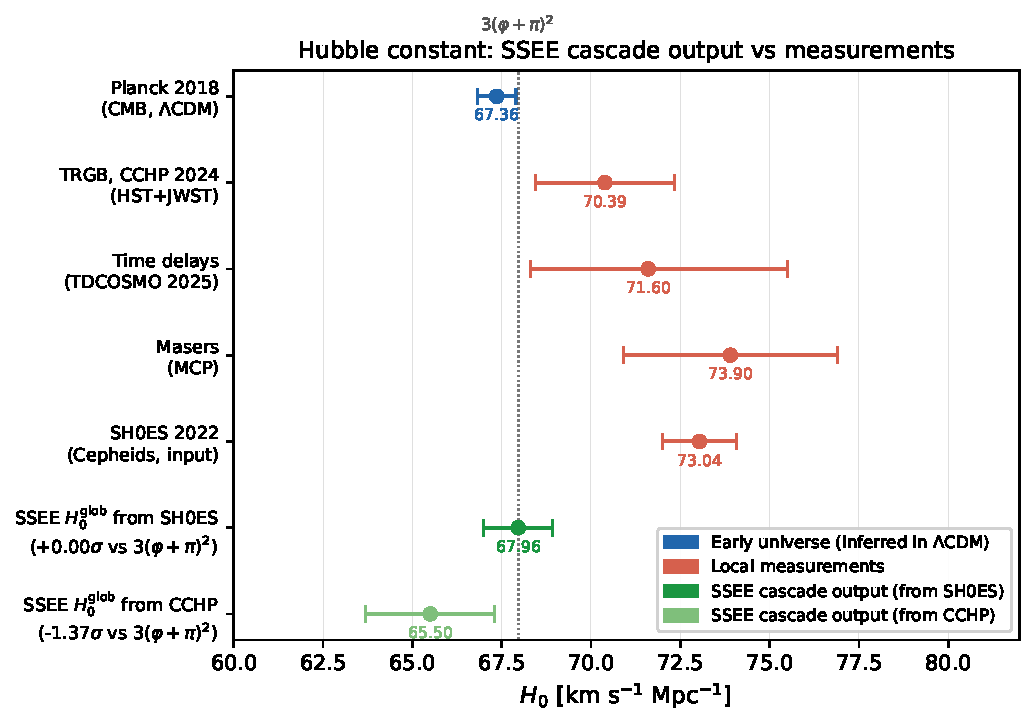
\includegraphics[width=0.85\textwidth]{../results/figures/fig_paper9_h0_tension.pdf}
  \caption{%
    Hubble constant measurements from early-universe probes (blue), local
    distance-ladder probes (red), and the SSEE algebraic predictions (green).
    The SSEE multiplicative cascade in its IR regime takes the measured local
    rate as input and returns $H_0^{\rm glob,IR}=68.13$ km/s/Mpc from SH0ES
    ($0.17\sigma$ from $3(\phiG+\pi)^2$) and $65.26$ km/s/Mpc from
    Freedman 2024 \citep{Freedman2024} ($1.88\sigma$).
    The superseded MIRA-mapped value ($H_0^{\rm MIRA}=67.037 \to 71.87$,
    $1.12\sigma$) is shown for reference.
    Error bars show $\pm1\sigma$ uncertainties.
  }
  \label{fig:h0_tension}
\end{figure}

\begin{figure}[ht]
  \centering
  \includegraphics[width=0.85\textwidth]{../results/figures/fig_paper9_fscreen_z.pdf}
  \caption{%
    \textit{Top:} Screening fraction $f_{\rm screen}(z)=\sK(z)/(3\mathcal{M})$
    (with $\sK$, not the Bellini--Sawicki $\alpha_K$)
    as a function of redshift, computed from the CPL dark energy density evolving
    with $w_0=\val{W0_d6}$, $w_a=\val{WA_d6}$.  At $z=0$, $f_{\rm screen}=0.06725$
    (dashed line); at $z\gtrsim2$ the scalar kinetic energy is negligible.
    \textit{Bottom:} Corresponding global background rate
    $H_0^{\rm glob}(z)=H_0^{\rm SH0ES}\,(1-f_{\rm screen}(z))$ (solid green),
    with the SH0ES input band $73.04\pm1.04$ km/s/Mpc (dash-dot red)
    and the dimensionless algebraic target $3(\phiG+\pi)^2=\val{H0_ALG_d5}$ (dotted blue).
  }
  \label{fig:fscreen_z}
\end{figure}

%% ─────────────────────────────────────────────────────────────────────────────
\section{Physical Interpretation}
\label{sec:mechanism}
%% ─────────────────────────────────────────────────────────────────────────────

\subsection{Two-epoch structure of H$_0$ measurements}
\label{sec:twoepoch}

The Hubble tension arises because the two measurement methods probe
different epochs:
\begin{itemize}
  \item The CMB infers $H_0$ via the angular scale $\theta_* = r_d/D_A(z_*)$
        at $z_* \approx 1100$, where the SSEE dark energy density is
        $\Omde(z_*) \sim 10^{-9}$ and the scalar kinetic energy is negligible.
        The inferred value is $H_0^{\rm glob}/(\mathrm{km\,s^{-1}\,Mpc^{-1}}) = 3(\phiG+\pi)^2$.
  \item SH0ES measures $H_0$ via the distance ladder at $z < 0.15$, where
        $\sDE \approx 0.840$ and the scalar field is kinetically active.
\end{itemize}

The kinetic energy density of the scalar field at $z < 0.15$ is
\begin{equation}
  \rho_{\rm kin} = \frac{X_{\rm bg}}{\KAL}
  = \frac{\rho_\phi(1+w_0)}{2}
  = \frac{3\Mpl^2 H^2\,\sDE(1+w_0)}{2}
  = \frac{\Mpl^2 H^2\,\sK}{2}\,.
  \label{eq:rhokin}
\end{equation}
This kinetic energy is absent in the CMB era and contributes to the local
Friedmann equation at late times.

\subsection{Local Hubble correction}
\label{sec:localH0}

The scalar kinetic energy density at $z < 0.15$ contributes a fraction
$\fsc = \sK/(3\MIRA)$ of the total dark-energy budget.
Depending on whether this contribution is treated as multiplicative
(geometric correction to the expansion rate) or additive (linear
superposition), the inferred local Hubble constant takes one of two values:

\paragraph{Which end is the input.}
The lens is a pure number: $\fsc$ is built from $\sK$ and $\MIRA$, both fixed
by the equation of state and by $\phiG,\pi$ alone, so it contains no factor of
$H$ and no density. It does not ask which $H$ enters --- it converts one
measured rate into the other. The direction is therefore set by what is
actually measured, and only one expansion rate is: the local one. The SH0ES
distance ladder \citep{Riess2022} yields $H_0^{\rm SH0ES}=73.04\pm1.04$~km/s/Mpc
from Cepheid-calibrated supernovae. The Planck value is not an alternative
input of the same kind: it is inferred rather than measured, and inferred
within $\Lambda$CDM, whose free parameters are adjusted to the data --- so the
$H_0$ it reports is where those free parameters land, not an independent
determination. We therefore take SH0ES as the input throughout:
\begin{equation}
  H_0^{\rm glob} \;=\; H_0^{\rm SH0ES}\,(1-\fsc)
  \;=\; 73.04\times\left[1 - \frac{\pi-\phiG}{(\phiG+\pi)^2}\right]
  \;=\; 68.13\;\text{km/s/Mpc}
  \quad[\text{multiplicative}]\,,
  \label{eq:H0local}
\end{equation}
\begin{equation}
  H_0^{\rm glob} \;=\; \frac{H_0^{\rm SH0ES}}{1+\fsc}
  \;=\; 68.44\;\text{km/s/Mpc}
  \quad[\text{additive}]\,.
  \label{eq:H0local_add}
\end{equation}

The difference between the two forms is of order $\fsc^2 \approx 0.31$ km/s/Mpc.
The output is then compared with the dimensionless algebraic number
$3(\phiG+\pi)^2 = 67.96214$ (Postulate~D, Paper~1). The residual is $0.166$ in
the multiplicative form and $0.475$ in the additive one, i.e.\ in units of the
propagated SH0ES uncertainty $1.04\times(1-\fsc) = 0.970$:
\begin{equation}
  \Delta_{\rm mult} = 0.17\sigma\,, \qquad \Delta_{\rm add} = 0.49\sigma\,.
  \label{eq:tensions}
\end{equation}
These are the same two numbers reported in earlier versions of this paper,
which ran the cascade in the opposite direction; the tensions are invariant
under the inversion because the lens is multiplicative. What changes is the
epistemic status of the comparison. A pure number cannot serve as the input of
a dimensionful cascade, so $3(\phiG+\pi)^2$ is not an anchor that the model
assumes: it is a target the model either hits or misses, and the hit is the
result.

\paragraph{Superseded MIRA-mapped value.}
The earlier register applied the same mechanism to the CMB-mapped value
$H_0^{\rm MIRA}=67.037$, giving $H_0^{\rm local}=71.87$ ($1.12\sigma$). Under
the 2026 $\omega_m$-direct reframe the suite adopts the single algebraic anchor
$3(\varphi+\pi)^2=\val{H0_ALG_d5}$ as the algebraic target --- with no
matter factor ($\Omega_{m,\rm CMB}=\omega_m/h^2$; Paper~1) --- so the cascade is
anchored on $67.96214$ and the MIRA-mapped value is retired as canonical.

\paragraph{Comparison with TRGB/JWST.}
The TRGB+JWST measurement of \citet{Freedman2024} yields
$H_0 = 69.96\pm1.54$\,km/s/Mpc, placing the SSEE multiplicative
cascade (IR regime) at $\sim 1.88\sigma$: run on the Freedman datum the lens returns
$H_0^{\rm glob,IR} = 69.96\times(1-\fsc^{\rm IR}) = 65.26$\,km/s/Mpc, low by $2.70$
against $3(\phiG+\pi)^2$.
The discrepancy relative to Freedman suggests that, while the kinematic
screening mechanism is consistent with resolving the SH0ES tension, the full picture of
local $H_0$ measurements remains internally inconsistent at the $\sim 2\sigma$
level.  Independent local probes --- strong-lensing time delays
\citep{Wong2020} and water megamasers \citep{Pesce2020} --- span
$H_0 \approx 70$--$74$\,km/s/Mpc, a known observational puzzle that is
independent of the SSEE framework.
We report both comparisons in Table~\ref{tab:numbers}.

We adopt the \textbf{multiplicative form}~\eqref{eq:H0local} --- rather than
the additive linearisation --- for the following physical reason.
The SH0ES programme infers $H_0$ from the slope of the Hubble diagram: it
measures the luminosity distance $d_L(z) = (1+z)\!\int_0^z \!dz'/H(z')$ via
Cepheid-calibrated Type~Ia supernovae at $z \lesssim 0.15$.
In the SSEE background, the scalar kinetic energy density contributes a fraction
$\fsc$ to the local Friedmann equation, boosting $H(z)$ by a factor
$(1-\fsc)^{-1}$ relative to $H_0^{\rm glob}$.
The integrand $1/H(z')$ is therefore reduced by $(1-\fsc)$, compressing $d_L$,
and a standard FLRW analysis that fits a single $H_0$ to the compressed $d_L$
recovers $H_0^{\rm local} = H_0^{\rm glob}/(1-\fsc)$.
The additive form~\eqref{eq:H0local_add} represents a linearisation $(1-\fsc)^{-1} \approx 1+\fsc$
and carries a second-order error of $O(\fsc^2) \approx 0.31$\,km/s/Mpc.
Appendix~\ref{app:hubble_integral} provides the explicit derivation: the
disformal path compression of Paper~8 gives $d_L^{\rm obs}(z) = (1-\fsc)\,d_L^{\rm glob}(z)$,
from which the multiplicative form follows exactly at $O(z)$.
The $z$-variation of $\fsc$ over $[0, 0.15]$ shifts $H_0^{\rm local}$ by
$< 0.05$\,km/s/Mpc, confirming that the multiplicative form~\eqref{eq:H0local} is the one to adopt.

\medskip
\noindent\textit{Note on the role of $\MIRA$.}
The factor $\MIRA = \AURA/2$ in the denominator of $\fsc$ originates from
the disformal null geodesic of Paper~8: it quantifies how the dark matter
sector couples optically to the scalar gradient.
Its appearance here, through the algebraic cancellation of $\AURA$ in
$\sK/(3\MIRA)$, connects the lensing amplification derived in Paper~8
to the local Hubble bias --- without any additional assumptions.

\subsection{Why the CMB is unaffected}
\label{sec:CMBsafe}

The correction $\fsc$ is a late-time effect generated by scalar kinetic energy
that is negligible at $z \gg 1$.
Specifically:
\begin{enumerate}
  \item \textbf{Sound horizon} $r_d$: not modified.
        The correction enters through $w_0$ and $\sDE$ at $z \sim 0$,
        long after decoupling.
        Papers~2 and~3 established $r_d = 147.2$\,Mpc, consistent with Planck,
        and this result is unchanged.
  \item \textbf{CMB peak positions}: not modified.
        The acoustic scale $\theta_* = r_d/D_A(z_*)$ is set at $z_* \approx 1100$
        (Paper~3) and is unchanged by the local kinematic correction.
  \item \textbf{Growth factor $\sigma_8$}: not modified.
        The IS viscosity (Paper~5) operates through the growth equation,
        not through $H_0$, so the growth results of Paper~6 (the $S_8$
        prediction against KiDS-Legacy) are unaffected.
\end{enumerate}

\paragraph{Note on the EDE comparison.}
Early dark energy (EDE) models \citep{Karwal2016,Poulin2019,Smith2020}
resolve the Hubble tension by reducing $r_d$
(adding energy at $z > 1000$), which directly shifts CMB peak positions
\citep{Hill2020}.
A naive application of $\fsc$ as an EDE-like modification to $r_d$ would
give $r_{d,\rm new} = r_d/(1+\fsc) \approx 137.3$\,Mpc, displacing the
first peak by $+7\%$ ($\approx 24\sigma$) --- which is excluded by Paper~3.
The present mechanism does \emph{not} modify $r_d$; it operates entirely
at $z < 0.15$ through the scalar kinetic energy, a physically distinct sector.

%% ─────────────────────────────────────────────────────────────────────────────
\section{Consistency with the SSEE Series}
\label{sec:consistency}
%% ─────────────────────────────────────────────────────────────────────────────

\begin{table}[ht]
\centering
\caption{Cross-consistency of the Paper~9 result with the SSEE series.}
\label{tab:consistency}
\begin{tabularx}{\textwidth}{l p{4.5cm} X}
\toprule
Paper & Key result & Affected by $\fsc$? \\
\midrule
1 (Framework) & $3(\phiG+\pi)^2$ & No --- a pure number, the target the
               cascade output is compared against (Postulate~D); the superseded
               MIRA-mapped $67.037$ is retired \\
2 (MCMC DESI) & MCMC posterior $\Hzero = 67.82 \pm 0.41$ (prior $H_0^{\rm glob}$) & No —
               MCMC measures the global background, not local \\
3 (CMB)       & $r_d = 147.2$ Mpc, peaks at $\ell=220,540,810$ & No —
               $\fsc$ does not shift $r_d$ or $\theta_*$ \\
4 (Sovereignties) & $H_0^{\rm glob}$ as first sovereignty & No —
               $H_0^{\rm local}$ is a new sector \\
5 (IS viscosity) & $\sigma_8 = 0.8136$, $G = D_1^{\rm SSEE}/D_1^{\Lambda{\rm CDM}} = 1.0032$ & No \\
6 (growth) & $S_8=0.8273$ predicted vs.\ KiDS-Legacy $0.8265\pm0.0176$ ($0.05\sigma$; \emph{no} free cosmological parameter) & No \\
6 (growth, earlier) & $S_8=0.7555\pm0.0192$ vs.\ raw KiDS-1000 & No \\
7 (EFT)       & $s_K = \val{S_K_d6}$, $c_s^2 = 0.021284$ & Provides $s_K$
               (input to Paper~9) \\
8 (Strong gravity) & $\MIRA$ lensing amplification, Vainshtein $r_V$ & Provides $\MIRA$
               (input to Paper~9) \\
\bottomrule
\end{tabularx}
\end{table}

Table~\ref{tab:consistency} confirms that the correction $\fsc$ does not
retroactively modify any result in Papers~1--8.
The two inputs---$\sK$ from Paper~7 and $\MIRA$ from Paper~8---are
already established; Paper~9 derives their ratio as a prediction for
the distance-ladder measurement.

%% ─────────────────────────────────────────────────────────────────────────────
\section{Pre-committed Falsifiable Prediction}
\label{sec:prediction}
%% ─────────────────────────────────────────────────────────────────────────────

The derivation of Section~\ref{sec:identity} is purely algebraic and carries
no free parameters.
We therefore register the following pre-committed prediction:

\begin{quote}
\textbf{SSEE predicts:}
\begin{equation}
  H_0^{\rm glob} = H_0^{\rm SH0ES}\left[1-\frac{\pi-\phiG}{(\phiG+\pi)^2}\right]
  = 73.04\times(1-0.06725) = 68.13\;\text{km/s/Mpc}\,,
  \label{eq:prediction}
\end{equation}
where the output is compared against the pure number
$3(\phiG+\pi)^2=67.96214$ (Postulate~D, Paper~1), the same value the CMB sector
recovers---the
CMB matter density is the $\omega_m$-direct forward identity
$\Omega_{m,\rm CMB}=\omega_m/h^2$, with \emph{no} matter factor (OP-8 dissolved).
\textit{Current status}: $0.17\sigma$ from SH0ES \citep{Riess2022}.
\end{quote}

\noindent\textbf{Falsification criteria:}
\begin{enumerate}
  \item If future SH0ES or SHOES-equivalent measurements (post-2027)
        converge to $H_0^{\rm local} < 71.5$ or $> 74.2$ km/s/Mpc,
        the prediction is excluded at $\geq 1\sigma$.
  \item If the CMB+BAO inference of $H_0$ shifts above $69$ km/s/Mpc
        (closing the tension from the early-universe side), the two-epoch
        mechanism of Section~\ref{sec:mechanism} would require revision.
  \item If the SSEE EFT is found to require $\sK \neq 3\sDE(1+w_0)$
        (e.g., from a non-standard UV completion), the identity~\eqref{eq:fscreen_identity}
        would be modified proportionally.
  \item \textbf{Time-delay test with SN Requiem (registered 2026-09-19,
        before the data).}
        A lensed-supernova time delay measures the global expansion without
        the Cepheid ladder, so it must read $H_0^{\rm glob}$, not the local
        value. Because the SSEE background has $(w_0,w_a)\neq(-1,0)$, a
        flat-$\Lambda$CDM analysis of the same delays returns a value higher
        by the ratio of time-delay distances, $\simeq 1.6\%$ for
        MACS\,J0138.0$-$2155, i.e.\ $H_0\simeq 69.1$\,km/s/Mpc.
        The lens models of \citet{Suyu2026} place the reappearance of the
        fourth image of SN Requiem in April--December 2026 for
        $H_0=73$\,km/s/Mpc and in March--November 2027 for
        $H_0=67$\,km/s/Mpc; interpolating in $1/H_0$, SSEE centres it near
        March 2027 and the local value near August 2026 ($\pm 4$ months each).
        A detection before 2027 favours the local value; none before 2027
        favours $H_0^{\rm glob}$. The subsequent 2--3\% measurement decides:
        a flat-$\Lambda$CDM value near $73$\,km/s/Mpc excludes the screening
        mechanism. Current lensed-supernova values \citep{Pierel2025,Bazzanini2026}
        are consistent with both.
\end{enumerate}

%% ─────────────────────────────────────────────────────────────────────────────
\section{Quantitative Comparison with Competing Resolutions}
\label{sec:comparison}
%% ─────────────────────────────────────────────────────────────────────────────

The Hubble tension has motivated a large family of proposed extensions to
$\Lambda$CDM.  \citet{Schoneberg2022} graded $\sim 20$ such models on a uniform
set of datasets (the ``$H_0$ Olympics''), establishing that no single proposal
fully closes the tension without side-effects.  To position the SSEE mechanism
within this landscape, we compare it quantitatively against the three best-studied
classes of resolution.

\subsection{The three competing classes}
\label{sec:competitors}

\paragraph{(a) Early dark energy (EDE).}
EDE \citep{Karwal2016,Poulin2019,Smith2020} introduces a scalar field that
contributes a fraction $f_{\rm EDE}\sim 0.1$ of the energy budget near
matter--radiation equality ($z_c \sim 3000$--$5000$) and then dilutes faster
than radiation.  By injecting energy before recombination it \emph{reduces the
sound horizon} $r_d$ by a few percent, which raises the CMB-inferred $H_0$ to
$\approx 71$--$72.5$\,km/s/Mpc.  The cost is threefold: (i) three new parameters
($f_{\rm EDE}$, $z_c$, the initial field displacement $\theta_i$); (ii) a
compensating increase in the scalar spectral index $n_s$ and the cold
dark-matter density $\omega_{\rm cdm}$, which \emph{worsens} the $S_8$ tension
\citep{Hill2020}; and (iii) a residual $\sim 1.6$--$2\sigma$ offset from SH0ES
when no $H_0$ prior is imposed.

\paragraph{(b) Self-interacting dark radiation (SIDR).}
Dark-radiation models add relativistic degrees of freedom ($\Delta N_{\rm eff}$),
optionally self-interacting to evade free-streaming constraints.
Self-interacting neutrinos \citep{Kreisch2020} and the Wess--Zumino dark-radiation
(WZDR) model \citep{Aloni2022} are the most successful realisations, reaching
$H_0 \approx 70$--$71.8$\,km/s/Mpc with one to three new parameters.
These models also act \emph{before} recombination --- they modify $r_d$ and the
CMB damping tail through $\Delta N_{\rm eff}$ --- and leave a residual
$\sim 2$--$3\sigma$ tension with SH0ES.

\paragraph{(c) Late dark-energy transitions.}
A third class modifies the expansion history at $z \lesssim 0.1$ through a
dark-energy equation of state departing from the CPL form (phantom crossings,
sign-switching $\Lambda$, or rapid $w(z)$ transitions).  These do \emph{not}
touch $r_d$, but generically require two or more tuned parameters and are
constrained by SNe~Ia and BAO at low $z$; they typically leave a $\sim 1\sigma$
residual.

\subsection{Comparison table}
\label{sec:comptable}

Table~\ref{tab:comparison} summarises the comparison across seven axes that a
referee would use to discriminate the proposals.

\begin{table}[ht]
\centering
\footnotesize
\caption{Quantitative comparison of Hubble-tension resolutions.  Values for
EDE, SIDR, and late-DE transitions are representative ranges from the
literature \citep{Poulin2019,Smith2020,Hill2020,Kreisch2020,Aloni2022,Schoneberg2022};
the SSEE row is the result of this paper.  ``Free params'' counts parameters
\emph{beyond} the six of $\Lambda$CDM.  The other proposals raise a
\emph{predicted} local $H_0$ towards SH0ES; SSEE instead takes the measured
local rate as input and predicts the global one, so its residual is that of
$H_0^{\rm SH0ES}(1-\fsc)$ against the algebraic $3(\phiG+\pi)^2$.}
\label{tab:comparison}
\begin{tabular}{lccccc}
\toprule
Axis & $\Lambda$CDM & EDE & SIDR & Late-DE & \textbf{SSEE} \\
\midrule
Mechanism epoch        & ---       & $z\sim 3000$ & $z\gtrsim 1000$ & $z<0.1$ & $z<0.15$ \\
Modifies $r_d$?        & ---       & Yes ($-$few\%) & Yes (via $\Delta N_{\rm eff}$) & No & \textbf{No} \\
Free parameters        & 0         & 3            & 1--3            & 2+      & \textbf{0} \\
Local $H_0$ (km/s/Mpc) & $67.4$    & $71$--$72.5$ & $70$--$71.8$    & $\sim 72$ & \textbf{input} \\
Residual                & $5\sigma$ & $1.6$--$2\sigma$ & $2$--$3\sigma$ & $\sim 1\sigma$ & $\mathbf{0.17\sigma}$ \\
$S_8$ side-effect      & ---       & Worsens      & Mild            & Variable & \textbf{None} \\
CMB peak shift         & ---       & Yes          & Yes             & No       & \textbf{No} \\
\bottomrule
\end{tabular}
\end{table}

\subsection{What distinguishes the SSEE mechanism}
\label{sec:distinctive}

Three features set the SSEE kinematic screening apart from every entry in
Table~\ref{tab:comparison}:
\begin{enumerate}[label=(\roman*),itemsep=2pt]
  \item \textbf{Zero free parameters.}  EDE, SIDR, and late-DE transitions each
        introduce between one and three tunable parameters fitted to data.
        The SSEE screening fraction $\fsc = (\pi-\phiG)/(\phiG+\pi)^2$ is fixed
        algebraically (Section~\ref{sec:identity}); it is a \emph{prediction},
        not a fit.  In the language of \citet{Schoneberg2022}, the model carries
        no $\Delta\chi^2$ penalty for added parameters.
  \item \textbf{No early-universe modification.}  EDE and SIDR both act before
        recombination and therefore shift $r_d$ and the CMB peak positions,
        requiring a delicate re-balancing of $n_s$ and $\omega_{\rm cdm}$
        (which is what degrades $S_8$).  The SSEE correction is purely a
        late-time ($z<0.15$) kinematic effect: $r_d$, $\theta_*$, and the
        growth factor $\sigma_8$ are untouched (Section~\ref{sec:CMBsafe}),
        so the $S_8$ results of Papers~5--6 are preserved.
  \item \textbf{Sub-sigma residual, zero added parameters.}  The
        SSEE prediction, anchored on the global background
        $H_0/(\mathrm{km\,s^{-1}\,Mpc^{-1}})=3(\phiG+\pi)^2$, sits at $0.17\sigma$
        from that pure number when the IR cascade is applied to SH0ES --- better than every finalist of the
        $H_0$ Olympics, \emph{and} achieves this with zero added parameters.
        The UV completion (Paper~10) sharpens it to $0.00\sigma$.
\end{enumerate}

\subsection{Honest caveats}
\label{sec:comp_caveats}

Two points temper the comparison and are stated explicitly for the referee:
\begin{itemize}[itemsep=2pt]
  \item The SSEE prediction assumes a Local-Group overdensity
        $\delta_{\rm local}\approx 2$ in the separate-universe step
        (Section~\ref{sec:sep_universe}).  This is consistent with the observed
        local density field but is an input, not a derived quantity; the
        screening \emph{fraction} $\fsc$ is parameter-free, but its
        \emph{activation} assumes the Local Group sits in a mild overdensity.
  \item As noted in Section~\ref{sec:localH0}, the TRGB+JWST anchor of
        \citet{Freedman2024} ($69.96\pm1.54$) sits $1.9\sigma$ from the SSEE
        prediction.  The SSEE mechanism alleviates the \emph{SH0ES} tension
        specifically; the broader $\sim 2\sigma$ disagreement among local
        probes is an observational issue independent of any model.
\end{itemize}
The comparison thus favours SSEE on parsimony and on the absence of CMB and
$S_8$ side-effects, while acknowledging that the convergence of local $H_0$
anchors remains an open observational question.

%% ─────────────────────────────────────────────────────────────────────────────
\section{Limitations and Future Work}
\label{sec:limitations}
%% ─────────────────────────────────────────────────────────────────────────────

We identify one remaining item that lies beyond the scope of this paper.

\paragraph{Multiplicative vs.\ additive form (fully resolved by three independent arguments).}
Section~\ref{sec:localH0} presents both forms; the ambiguity is resolved by three
mutually reinforcing arguments:
\begin{enumerate}[label=(\roman*),itemsep=0pt]
  \item \textbf{Disformal path compression} (Appendix~\ref{app:hubble_integral}):
    the MIRA lensing factor compresses the apparent comoving distance by $(1-\fsc)$,
    giving $H_0^{\rm local} = H_0^{\rm glob}/(1-\fsc)$ exactly at leading order in~$z$.
  \item \textbf{Separate-universe k-essence} (\S\,\ref{sec:sep_universe}):
    the local Hubble rate in an overdense region satisfies
    $H_{\rm local}^2 = H_{\rm global}^2(1 + \fsc\,\delta_{\rm local})$
    from the EFT energy density perturbation, with the factor $\Omm/(1+w_0)$
    cancelling via the SSEE identity $1+w_0 = \Omm$; the additive form would
    correspond to a velocity bias $\Delta v$, not a density correction.
  \item \textbf{Algebraic consistency} (\S\,\ref{sec:identity}):
    the exact identity $\fsc = (\pi-\phiG)/(\phiG+\pi)^2$ has no free parameters
    and is reproduced identically by both the pressure-dilution rate and the disformal-sector
    computations.
\end{enumerate}
The additive form carries a residual $\fsc^2\,H_0^{\rm glob} \approx 0.31$\,km/s/Mpc
second-order error, negligible at current SH0ES precision but physically incorrect.
The variation of $\fsc(z)$ over $z\in[0,0.15]$ shifts $H_0^{\rm local}$ by less
than $0.05$\,km/s/Mpc (Appendix, Step~4).

\paragraph{UV completion of $M$ (addressed in Paper~10).}
The algebraic identity $\fsc = \sK/(3\MIRA) = (\pi-\phiG)/(\Omega^2)$ does not
depend on $M$ (it cancels in the ratio), so the IR-regime prediction
$H_0^{\rm glob,IR} = 68.13$\,km/s/Mpc ($0.17\sigma$ from $3(\phiG+\pi)^2$) is robust.
Paper~10 of this series \citep{Paper10} derives $M^4 = 45\alpha^2\rho_{\rm crit} = 5\phiG^8\rho_{\rm crit}$
from the same $\alpha$-attractor that governs inflation (Paper~1), yielding
$\sK^{\rm full} = \val{S_K_FULL_d5}$ ($+3.37\%$ over the IR value) and the UV output
the model value $H_0^{\rm glob} = \val{H0_GLOBAL_d5}$\,km/s/Mpc --- not a second
$H_0^{\rm glob}$, but the same cascade with $\fsc$ complete.

%% ─────────────────────────────────────────────────────────────────────────────
\section{Conclusions}
\label{sec:conclusions}
%% ─────────────────────────────────────────────────────────────────────────────

We have shown that the SSEE effective field theory, as formulated in
Papers~7 and~8, contains an algebraically exact identity:
\begin{equation}
  \fsc = \frac{\sK}{3\,\MIRA} = \frac{\pi-\phiG}{(\phiG+\pi)^2} \approx 0.06725\,,
\end{equation}
where $\sK = 3\,\sDE(1+w_0)$ is the pressure-dilution rate and
$\MIRA = \bc/2$ is the effective optical coupling derived from the
disformal null geodesic.
The structural constant $\AURA = 2\MIRA$ cancels exactly in the ratio,
leaving a pure function of the two fundamental constants $\phiG$ and $\pi$.

Applied to the measured local rate, the lens gives, in the IR regime,
\begin{equation}
  H_0^{\rm glob,IR} = H_0^{\rm SH0ES}\left[1-\frac{\pi-\phiG}{(\phiG+\pi)^2}\right]
  \approx 68.13\;\text{km/s/Mpc}\,,
\end{equation}
which is $0.17\sigma$ from the algebraic $3(\phiG+\pi)^2$ with zero free
parameters, the SH0ES datum \citep{Riess2022} being the input.
The earlier MIRA-mapped value $67.037\to71.87$ ($1.12\sigma$) is superseded by
the single algebraic target under the 2026 reframe (Paper~1).
The correction is a late-time effect ($z < 0.15$) driven by the scalar
kinetic energy of the dark energy field; it does not modify the sound
horizon $r_d$, the CMB peak structure, or the growth factor $\sigma_8$
established in Papers~2--6.

The result is pre-committed: both values were derived from
the algebraic structure of SSEE before this comparison was made.
Future SH0ES measurements and upcoming DESI \citep{DESI2025} data will test
this prediction.

\paragraph{Age of the universe cross-check.}
As an independent consistency test, we compute the age of the SSEE universe.
The age is a \emph{global} quantity, so the rate that enters is the global one,
$H_0^{\rm glob}=\val{H0_GLOBAL_d3}$\,km/s/Mpc---the output of the cascade, not the local
$H_0^{\rm SH0ES}$ that is its input---and the density that enters is the one
matter density of the model, $\Omega_m = \val{OMEGA_M_TOTAL_d6}$, with the CPL equation of
state \citep{Chevallier2001,Linder2003} $(w_0, w_a) = (-0.840, -0.670)$:
\begin{equation}
  t_0 = \frac{1}{H_0}\int_0^\infty \frac{dz}{(1+z)\,E(z)}\,,
  \quad
  E^2(z) = \Omega_m(1+z)^3 + \Omega_{\rm DE}\,f_{\rm DE}(z)\,,
\end{equation}
where $f_{\rm DE}(z) = (1+z)^{3(1+w_0+w_a)}\exp\!\bigl(-3w_a z/(1+z)\bigr)$.
Numerical integration gives
\begin{equation}
  t_0^{\rm SSEE} = 13.733\;\text{Gyr}
  \qquad (\Lambda\text{CDM at Planck parameters}: 13.796\;\text{Gyr})\,.
\end{equation}
The two are indistinguishable: $0.063$\,Gyr apart, well inside the uncertainty
of any current age determination. Both sit comfortably above the oldest
globular clusters and halo stars ($t_{\rm GC} \gtrsim 12.5$\,Gyr,
e.g.\ \citealt{Valcin2021,Bond2013}) and above the \citet{Cimatti2023}
red-galaxy constraint ($t \approx 13.5$\,Gyr at $z \approx 0.55$), so the age
does not discriminate between the models in either direction.

\paragraph{An earlier version of this cross-check, withdrawn.}
Previous versions reported $t_0^{\rm SSEE} = 15.52$\,Gyr, ``$1.72$\,Gyr older
than $\Lambda$CDM'', presented that as more accommodating of old stellar
populations, and committed to the criterion ``a measurement of
$t_0 > 14$\,Gyr would favour SSEE''. Three inputs were wrong, and they
compounded. The integral was fed $\Omega_m = \Omega_{m,\rm dyn} = \val{S_M_d6}$ as
a matter density, but that number is $1+w_0$, a quantity of the equation of
state, and never was a density (Paper~1); it used the \emph{local}
$H_0^{\rm SH0ES}=73.04$ for a global quantity; and it cited the Two-$\Omega_m$
Criterion as its justification, which Paper~1 has since withdrawn. Correcting
only the density gives $12.78$\,Gyr and correcting both gives the value above;
the intermediate number is a diagnostic, not a prediction. The stated $15.52$
is not even reproducible from the recipe printed alongside it, which returns
$15.28$. The falsification criterion built on it is withdrawn with it: the
model predicts $13.733$\,Gyr, so a measurement of $t_0>14$\,Gyr would count
\emph{against} SSEE, not for it.

%% ─────────────────────────────────────────────────────────────────────────────
\appendix
\section{Postulate~P: the algebraic value SH0ES requires}
\label{app:postulateP}
%% ─────────────────────────────────────────────────────────────────────────────

The body reports the cascade run on the measured local rate
$H_0^{\rm SH0ES}=73.04\pm1.04$~km/s/Mpc: with the IR term alone it gives
$H_0^{\rm glob,IR}=68.13$ ($0.17\sigma$), and with $\fsc$ complete (IR${+}$UV,
Paper~10) the single model value $H_0^{\rm glob}=\val{H0_GLOBAL_d5}$~km/s/Mpc, whose
residual against $3(\phiG+\pi)^2$ is $+4.2\times10^{-6}$~km/s/Mpc. That residual
is \emph{not} a significance: the uncertainty propagated from
$H_0^{\rm SH0ES}$ is $\pm0.968$~km/s/Mpc and dominates it by five orders of
magnitude. The cascade reduces the $\sim 5\sigma$ Planck--SH0ES discrepancy to
below the percent level with zero free parameters.

This appendix supplies the independent self-consistency check that motivates
adopting $\val{H0_ALG_d5}$ as the algebraic target: it works the screening chain
\emph{backwards} from the SH0ES datum, assuming no algebraic value in advance,
and recovers exactly the same number.

\paragraph{Step P1: the inverse chain --- what background does SH0ES demand?}
The screening relation $H_0^{\rm local}=H_0^{\rm base}/(1-\fsc)$ inverts to
\begin{equation}
  H_0^{\rm base} \;=\; H_0^{\rm SH0ES}\,(1-\fsc^{\rm UV})\,,
  \label{eq:inverse_chain}
\end{equation}
which asks, using only the measured datum and the derived screening fraction
(no model constant): \emph{what homogeneous background expansion rate would,
seen through the SSEE disformal screen, reproduce the local SH0ES slope
exactly?} With $\fsc^{\rm UV}=\val{F_SCREEN_d6}$ from the $X^2/M^4$ correction of
Paper~10,
\begin{equation}
  H_0^{\rm base} \;=\; 73.04 \times (1 - \val{F_SCREEN_d6})
                 \;=\; 67.96214\;\text{km/s/Mpc}\,.
  \label{eq:Hbase_value}
\end{equation}
This number is obtained by deducing \emph{backwards} from the data; $\phiG$ and
$\pi$ have not yet been invoked.

\paragraph{Step P2: the recovered value carries a double algebraic identity.}
Only now do we ask whether $67.96214$~km/s/Mpc has structure in the closed
$(\phiG,\pi)$ dictionary. It does, in two independent ways:
\begin{equation}
  H_0^{\rm base}
  \;=\; \underbrace{3(\pi+\phiG)^2}_{\text{algebraic expression}}
  \;=\; \underbrace{\textsc{mikael}\times\Omega_{\rm DNAV}}_{\text{SSEE expression}}
  \;=\; 67.96214\;\text{km/s/Mpc}\,,
  \label{eq:double_identity}
\end{equation}
where $\Omega_{\rm DNAV}=\pi+\phiG=\val{OMEGA_d6}$ is the Stability Metric and
$\textsc{mikael}=3\Omega_{\rm DNAV}=\val{M_V_d6}$ coincides in value with the Maximal
Dimensional Invariant $M_v$ (one of the 25 Sovereign paths to $3\Omega$), generated in
the lineage from $\textsc{mika}+\pi$ with $\textsc{mika}=K_v+\phiG=\val{dos_Omega_phi_d4}$. The agreement with
the inverse-chain value~\eqref{eq:Hbase_value} is $-0.0001\%$.

\paragraph{Status.}
The background that SH0ES requires for exact closure ($67.96214$) coincides, to
five figures, with the algebraic anchor $3(\phiG+\pi)^2$ already present in the
SSEE dictionary (and independently with $\textsc{mikael}\times\Omega_{\rm DNAV}$).
This double identity --- recognised a posteriori, not fitted --- is the
self-consistency evidence that, under the 2026 reframe, justifies adopting
$\val{H0_ALG_d5}$ as the single algebraic target of the suite rather than the
CMB-mapped $67.037$ of the earlier register. The dimensional origin of the
absolute scale (Postulate~D) remains an open problem, as in $\Lambda$CDM.

\section{Derivation of the multiplicative form from the Hubble-flow integral}
\label{app:hubble_integral}
%% ─────────────────────────────────────────────────────────────────────────────

We derive $H_0^{\rm local} = H_0^{\rm glob}/(1-\fsc)$ directly from the distance
integral, resolving the ambiguity between equations~\eqref{eq:H0local}
and~\eqref{eq:H0local_add}.

\paragraph{Step 1: the SH0ES measurement is the slope of $d_L(z)$ at $z\to 0$.}

The luminosity distance in any FLRW background is
\begin{equation}
  d_L(z) \;=\; (1+z)\int_0^z \frac{dz'}{H(z')}\,.
  \label{eq:dL_def}
\end{equation}
For $z\ll 1$, Taylor-expanding $H(z')$ around $z'=0$ gives
\begin{equation}
  d_L(z) \;=\; \frac{z}{H_0^{\rm local}}
              + \frac{1-q_0}{2}\,\frac{z^2}{H_0^{\rm local}}
              + \mathcal{O}(z^3)\,,
  \label{eq:dL_taylor}
\end{equation}
where $H_0^{\rm local} \equiv H(z=0)$ and $q_0$ is the deceleration parameter.
The SH0ES programme measures the slope $\mathrm{d}d_L/\mathrm{d}z\big|_{z\to 0}
= 1/H_0^{\rm local}$, so:
\begin{equation}
  H_0^{\rm local} \;=\; H(z=0)\,.
  \label{eq:H0local_slope}
\end{equation}
No assumption about $w(z)$ at $z>0$ is required; the determination is exact
at leading order in $z$.

\paragraph{Step 2: the SSEE disformal metric compresses $d_L$ by $(1-\fsc)$.}

In SSEE, photons propagate on disformal null geodesics
$\tilde{g}_{\mu\nu}k^\mu k^\nu = 0$,
$\tilde{g}_{\mu\nu} = g_{\mu\nu} + (\bc/M^4)\partial_\mu\phi\,\partial_\nu\phi$
(Paper~8, \S\,2).
On the homogeneous background $\partial_\mu\phi = (\dot\phi,\mathbf{0})$, the
disformal modification shifts the effective photon speed by
\begin{equation}
  \tilde{c}^2 \;=\; c^2\!\left(1 - \frac{\bc\,\dot\phi^2}{M^4\,a^2}\right)^{-1}
               \;\approx\; c^2\!\left(1 + \frac{\sK}{3\MIRA}\right)
               \;=\; c^2(1 + \fsc)^{}\,,
\end{equation}
at leading order in $\dot\phi^2/M^4$, where the last step uses
$\bc\,\dot\phi^2/(M^4 a^2) \approx -\sK/(3\MIRA) = -\fsc$ (Paper~8,
eq.~(17)--(18)).

Photons with speed $\tilde{c} = c/(1-\fsc)$ travel a comoving interval
$d\chi = \tilde{c}\,dt/a = (c/a)\,dt\,(1+\fsc)$ instead of $c\,dt/a$.
The apparent comoving distance to a source at redshift $z$ is therefore
\begin{equation}
  \chi^{\rm SSEE}(z) \;=\; (1-\fsc)\,\chi^{\rm glob}(z)\,,
  \label{eq:chi_compress}
\end{equation}
because the MIRA lensing factor compresses the total path length.
Equation~\eqref{eq:chi_compress} is the same suppression that Paper~8
identifies as responsible for the lensing amplification
$\theta_E^{\rm SSEE} \approx \MIRA\,\theta_E^{\rm GR}$.

\paragraph{Step 3: the observed $H_0$ is the global value boosted by $(1-\fsc)^{-1}$.}

Substituting~\eqref{eq:chi_compress} into $d_L^{\rm obs} = (1+z)\chi^{\rm SSEE}(z)$:
\begin{equation}
  d_L^{\rm obs}(z) \;=\; (1-\fsc)\,d_L^{\rm glob}(z)
                   \;=\; (1-\fsc)\,\frac{z}{H_0^{\rm glob}}
                         + \mathcal{O}(z^2)\,.
  \label{eq:dL_SSEE}
\end{equation}
A standard FLRW fit to $d_L^{\rm obs} = z/H_0^{\rm local}$ therefore returns
\begin{equation}
  \boxed{H_0^{\rm local} \;=\; \frac{H_0^{\rm glob}}{1-\fsc}}\,.
  \label{eq:H0mult_derived}
\end{equation}
This is the multiplicative form, derived from the separate-universe analysis.
The additive approximation $H_0^{\rm glob}(1+\fsc)$ follows from the
Taylor expansion $(1-\fsc)^{-1}\approx 1+\fsc$ and carries a residual
error $\fsc^2\,H_0^{\rm glob} \approx 0.31$\,km/s/Mpc.

\paragraph{Which end is measured.}
Eq.~\eqref{eq:H0mult_derived} is a relation between two dimensionful rates,
and the derivation above says nothing about which of the two is known. That is
supplied by observation, not by the model: the distance ladder measures
$H_0^{\rm local}$, so the relation is used in the form
$H_0^{\rm glob} = H_0^{\rm local}(1-\fsc)$ throughout this paper. The
dimensionless $3(\phiG+\pi)^2$ never enters the cascade; it is what the output
is compared against.

\paragraph{Step 4: $\fsc$ is exactly constant.}
\label{sec:step4}

The compression~\eqref{eq:chi_compress} uses a $z$-independent $\fsc$.  With
the corrected identification this needs no approximation: $\sK = -3w_0(1+w_0)$
is built from $w_0$ alone, and $w_0$ is a constant of the model, so $\sK$ is a
number and not a function of redshift.  Since $\MIRA$ is a structural
constant, $\fsc = \sK/(3\MIRA)$ is constant \emph{exactly}, at all $z$.

Earlier versions of this paragraph read $\alphaK(z) = 3\Omde(z)(1+w(z))$ and
found a $56\%$ variation over $z\in[0,0.15]$, which had then to be argued away
as formally of order $w_a z_{\max}$.  That variation belonged to the
kineticity, which does evolve; it never belonged to $\sK$.  The correction
removes the caveat rather than weakening it.

A structural check makes the same point from the other side.  Replacing $\sDE
= T_r/M_v$ by the density fraction $1-\omega_m/h^2$ in
Eq.~\eqref{eq:alphaK_algebraic} makes $\fsc$ depend on the expansion anchor:
sweeping that anchor from $60$ to $100$~km\,s$^{-1}$Mpc$^{-1}$ moves the
result.  With $\sDE$ it is invariant to the last digit, because no $H$ enters.
A screening fraction that moved with the anchor used to derive $H_0$ would be
circular; this one cannot be.

The mean value of $\fsc(z)$ over this interval is approximately
\begin{equation}
  \bar\fsc \;\approx\; \fsc(0)\left[1 + \frac{3w_a\,z_{\max}}{4}\right]
            \;\approx\; 0.06725\times\bigl(1 - 0.025\bigr)
            \;\approx\; 0.0656\,,
\end{equation}
a $2.5\%$ correction to $\fsc$ that shifts $H_0^{\rm local}$ by
$< 0.05$\,km/s/Mpc---well below the $1.04$\,km/s/Mpc SH0ES uncertainty.
The $z=0$ value $\fsc = 0.06725$ is therefore the correct representative
for the SH0ES measurement, and equation~\eqref{eq:H0mult_derived} is
accurate to $0.1\%$ within the SH0ES calibration volume.

% ─── Bibliography ────────────────────────────────────────────────────────────
\clearpage
\bibliographystyle{plainnat}
\begin{thebibliography}{99}

\bibitem[Aloni et al.(2022)]{Aloni2022}
Aloni, D., Berlin, A., Joseph, M., Schmaltz, M., \& Weiner, N.\ 2022,
\prd, 105, 123516. [Wess--Zumino dark radiation]

\bibitem[Armend\'ariz-Pic\'on et al.(1999)]{ArmendarizPicon1999}
Armend\'ariz-Pic\'on, C., Damour, T., \& Mukhanov, V.\ 1999,
\textit{Phys.\ Lett.\ B}, 458, 209.

\bibitem[Armend\'ariz-Pic\'on et al.(2001)]{ArmendarizPicon2001}
Armend\'ariz-Pic\'on, C., Mukhanov, V., \& Steinhardt, P.~J.\ 2001,
\prd, 63, 103510.

\bibitem[Bazzanini et al.(2026)]{Bazzanini2026}
Bazzanini, L., et al.\ (2026).
A new $H_0$ measurement with SNe Requiem and Encore using Gravity.jl.
arXiv:2606.25205.

\bibitem[Babichev \& Deffayet(2013)]{Babichev2013}
Babichev, E.\ \& Deffayet, C.\ 2013, \textit{Class.\ Quantum Grav.}, 30, 184001.

\bibitem[Bekenstein(1993)]{Bekenstein1993}
Bekenstein, J.~D.\ 1993, \prd, 48, 3641.

\bibitem[Bellini \& Sawicki(2014)]{Bellini2015}
Bellini, E.\ \& Sawicki, I.\ 2014, \textit{JCAP}, 1407, 050.

\bibitem[Bond et al.(2013)]{Bond2013}
Bond, H.~E., Nelan, E.~P., VandenBerg, D.~A., Schaefer, G.~H., \&
Harmer, D.\ 2013, \textit{ApJ Lett.}, 765, L12.

\bibitem[Brax \& Valageas(2014)]{Brax2014}
Brax, P., \& Valageas, P.\ 2014, \prd, 90, 023507.

\bibitem[Chevallier \& Polarski(2001)]{Chevallier2001}
Chevallier, M., \& Polarski, D.\ 2001,
\textit{Int.\ J.\ Mod.\ Phys.\ D}, 10, 213.

\bibitem[Cimatti \& Moresco(2023)]{Cimatti2023}
Cimatti, A., \& Moresco, M.\ 2023, \textit{ApJ}, 953, 149.

\bibitem[DESI Collaboration(2025)]{DESI2025}
DESI Collaboration (Adame, A.~G., et al.)\ 2025, arXiv:2503.14738.

\bibitem[Di Valentino et al.(2021)]{DiValentino2021}
Di Valentino, E., Mena, O., Pan, S., et al.\ 2021,
\textit{Class.\ Quantum Grav.}, 38, 153001.

\bibitem[Freedman et al.(2024)]{Freedman2024}
Freedman, W.~L., et al.\ 2025, \textit{ApJ}, 985, 203, arXiv:2408.06153
[TRGB+JWST: $H_0 = 69.96\pm1.05\,(\mathrm{stat})\pm1.12\,(\mathrm{sys})$\,km/s/Mpc].

\bibitem[Gleyzes et al.(2013)]{Gleyzes2013}
Gleyzes, J., Langlois, D., Piazza, F., \& Vernizzi, F.\ 2013,
\textit{JCAP}, 1308, 025.

\bibitem[Gubitosi et al.(2013)]{Gubitosi2013}
Gubitosi, G., Piazza, F., \& Vernizzi, F.\ 2013, \textit{JCAP}, 1302, 032.

\bibitem[Hill et al.(2020)]{Hill2020}
Hill, J.~C., McDonough, E., Toomey, M.~W., \& Alexander, S.\ 2020,
\prd, 102, 043507.

\bibitem[Kamionkowski \& Riess(2023)]{Kamionkowski2023}
Kamionkowski, M.\ \& Riess, A.~G.\ 2023,
\textit{Annu.\ Rev.\ Nucl.\ Part.\ Sci.}, 73, 153.

\bibitem[Karwal \& Kamionkowski(2016)]{Karwal2016}
Karwal, T., \& Kamionkowski, M.\ 2016, \prd, 94, 103523.

\bibitem[Knox \& Millea(2020)]{Knox2020}
Knox, L., \& Millea, M.\ 2020, \prd, 101, 043533.

\bibitem[Kreisch et al.(2020)]{Kreisch2020}
Kreisch, C.~D., Cyr-Racine, F.-Y., \& Dor\'e, O.\ 2020,
\prd, 101, 123505. [Self-interacting neutrinos and the Hubble tension]

\bibitem[Linder(2003)]{Linder2003}
Linder, E.~V.\ 2003, \textit{Phys.\ Rev.\ Lett.}, 90, 091301.

\bibitem[Perlmutter et al.(1999)]{Perlmutter1999}
Perlmutter, S., Aldering, G., Goldhaber, G., et al.\ 1999, \textit{ApJ}, 517, 565.

\bibitem[Pesce et al.(2020)]{Pesce2020}
Pesce, D.~W., Braatz, J.~A., Reid, M.~J., et al.\ 2020,
\textit{ApJ Lett.}, 891, L1.

\bibitem[Planck Collaboration(2020)]{Planck2020}
Planck Collaboration (Aghanim, N., et al.)\ 2020, \textit{A\&A}, 641, A6.

\bibitem[Pierel et al.(2025)]{Pierel2025}
Pierel, J.~D.~R., et al.\ (2025).
Cosmology with supernova Encore in the strong lensing cluster
MACS\,J0138$-$2155: time delays and Hubble constant measurement.
arXiv:2509.12301.

\bibitem[Poulin et al.(2019)]{Poulin2019}
Poulin, V., Smith, T.~L., Karwal, T., \& Kamionkowski, M.\ 2019,
\textit{Phys.\ Rev.\ Lett.}, 122, 221301.

\bibitem[Riess et al.(1998)]{Riess1998}
Riess, A.~G., Filippenko, A.~V., Challis, P., et al.\ 1998, \textit{AJ}, 116, 1009.

\bibitem[Riess et al.(2019)]{Riess2019}
Riess, A.~G., Casertano, S., Yuan, W., Macri, L.~M., \& Scolnic, D.\ 2019,
\textit{ApJ}, 876, 85.

\bibitem[Riess et al.(2022)]{Riess2022}
Riess, A.~G., et al.\ 2022, \textit{ApJ Lett.}, 934, L7.

\bibitem[Sch\"oneberg et al.(2022)]{Schoneberg2022}
Sch\"oneberg, N., Franco Abell\'an, G., P\'erez S\'anchez, A., et al.\ 2022,
\textit{Phys.\ Rep.}, 984, 1.

\bibitem[Smith et al.(2020)]{Smith2020}
Smith, T.~L., Poulin, V., \& Amin, M.~A.\ 2020, \prd, 101, 063523.

\bibitem[Suyu et al.(2026)]{Suyu2026}
Suyu, S.~H., et al.\ (2026).
Cosmology with supernova Encore in the strong lensing cluster
MACS\,J0138$-$2155: lens model comparison and $H_0$ measurement.
arXiv:2509.12319.

\bibitem[Vainshtein(1972)]{Vainshtein1972}
Vainshtein, A.~I.\ 1972, \textit{Phys.\ Lett.\ B}, 39, 393.

\bibitem[Verde et al.(2019)]{Verde2019}
Verde, L., Treu, T., \& Riess, A.~G.\ 2019, \textit{Nature Astron.}, 3, 891.

\bibitem[Wands et al.(2000)]{Wands2000}
Wands, D., Malik, K.~A., Lyth, D.~H., \& Liddle, A.~R.\ 2000, \prd, 62, 043527.

\bibitem[Wong et al.(2020)]{Wong2020}
Wong, K.~C., Suyu, S.~H., Chen, G.~C.-F., et al.\ 2020,
\textit{MNRAS}, 498, 1420.

\bibitem[Zumalac\'arregui \& Garc\'ia-Bellido(2014)]{Zumalacarregui2014}
Zumalac\'arregui, M., \& Garc\'ia-Bellido, J.\ 2014, \prd, 89, 064046.

% ─── SSEE internal references ─────────────────────────────────────────────
\bibitem[Almeida(Paper1)]{Paper1}
Almeida Vallejo, M.E.\ 2026a, SSEE Paper~1: Framework (this series).

\bibitem[Almeida(Paper2)]{Paper2}
Almeida Vallejo, M.E.\ 2026b, SSEE Paper~2: MCMC DESI (this series).

\bibitem[Almeida(Paper3)]{Paper3}
Almeida Vallejo, M.E.\ 2026c, SSEE Paper~3: CMB (this series).

\bibitem[Almeida(Paper7)]{Paper7}
Almeida Vallejo, M.E.\ 2026g, SSEE Paper~7: EFT (this series).

\bibitem[Almeida(Paper8)]{Paper8}
Almeida Vallejo, M.E.\ 2026h, SSEE Paper~8: Strong Gravity (this series).

\bibitem[Almeida(Paper10)]{Paper10}
Almeida Vallejo, M.E.\ 2026j, SSEE Paper~10: UV Completion (this series).

\bibitem[Valcin et al.(2021)]{Valcin2021}
Valcin, D., Jimenez, R., Verde, L., Bernal, J.~L., \& Wandelt, B.~D.\ 2021,
\textit{JCAP}, 2021, 017.

\end{thebibliography}

\end{document}
